\section{Procedural Textures}

Texturing, in general, is a method of adding more detail and realism to a 3D object, traditionally by projecting a 2D bitmap texture to its surface. This is a rather straight forwards process, but presents a number of problems that are difficult to overcome. Firstly, a bitmap texture has a fixed amount of detail; a pixel resolution. The resolution of an image can normally not be scaled up, although new research has made progress in that aspect much thanks to the advances in neural networks \cite{richard_2019_learned, li_2019_a}. However, even if the resolution is sufficient, bitmap textures are still inflexible as it is difficult to modify the underlying pattern without negatively affecting its overall appearance. Furthermore, bitmap textures require a considerable amount of storage space. Another hurdle that is often overlooked, is the inherent problem of projecting 2D texture coordinates $p_{2D} = (u,v)$ onto points on a 3D object's surface $p_{3D} = (x,y,z)$. This mapping process is a function from three dimensional points on an objects surface to two dimensional coordinates in a texture matrix and is often referred to as \textit{UV mapping}, see equation \ref{eq:UVMapping}, often introducing visible seams on the edges between object surfaces as in figure \ref{fig:BitmapVsProcedural}. 

\begin{equation}\label{eq:UVMapping}
    f(u,v) : \mathbb{R}^3 \mapsto \mathbb{N}^2
\end{equation}

Procedural textures are created using mathematical functions, often referred to as \textit{shaders} in computer graphics, that take the surface coordinates of the 3D object as input, as well as a set of $n$ parameters $\theta \in \mathbb{R}^n$ describing its appearance, and returns a color for the point $p_{3D} = (x,y,z)$ see equation \ref{eq:ProceduralMapping}. The parameters $\theta$ can be tweaked by the user to change the underlying patterns and colors, making them much more flexible than the static bitmap approach. 

\begin{equation}\label{eq:ProceduralMapping}
    f(x,y,z,\theta): \mathbb{R}^3, \mathbb{R}^n \mapsto \mathbb{R}^3
\end{equation}


\subsection{Function Composition}

Being functions means we can extend the functionality of procedural textures using \textit{function composition}, a basic mathematical operation taking two functions $f(x)$ and $g(x)$ as input and produces a new function $h(x) = f(g(x))$. While the final output of the procedural texture function should be the color of a point on a target object's surface, any output of any function $g(x)$ can be used as input to a procedural function $f(x)$. To understand how powerful function composition is when user with procedural textures, let $f(\vec{v}, \vec{w}, a)$ be a function of two vectors and a scalar mix factor that returns a weighted sum of both vectors, essentially mixing them. Let $g(x,y,z,a)$ be a function that returns an arbitrary sinusoidal pattern that depends on the input coordinates $(x,y,z)$ as well as a scaling factor $a$ and finally, let $r(x,y,z,\vec{\theta})$ be the main procedural texture function. We also define a red color vector and a green color vector, $c_r = (1.0,0.0,0.0)$ and $c_g = (0.0,0.3,0.0)$ where the elements represent the red, green and blue channels. The functions are defined in equation \ref{eq:ProceduralFunctionComposition} where $\odot$ denotes an element-wise multiplication operation.

\begin{equation}\label{eq:ProceduralFunctionComposition}
\begin{aligned}
    f(\vec{v}, \vec{w}, a) &= \vec{v} \odot (1 - a) + \vec{w} \odot a \\
    g(x,y,z,a) &= \sin(a \cdot x)\cdot \sin(a \cdot y)\cdot \sin(a \cdot z)  \\
    r(x,y,z,\vec{\theta}) &= f(c_r, c_g, g(x,y,z,\theta_0))
\end{aligned}
\end{equation}

Using $r$ as a procedural render function to texture a plane ($\forall z, z = 0$), we achieve 

\subsection{Noise}


\section{Automatic Differentiation}\label{sec:AutomaticDifferentiation}

A major reason why inverse rendering is a difficult problem, is because the rendering process needs to be differentiable in order to be inverted. The reason relates to our iterative optimization algorithm \textit{Gradient Descent}, explained in section \ref{sec:StochasticGradientDescent}, which uses the gradient of a function $f(x_0, x_1, ..., x_i)$, denoted $\nabla f$, defined as the collection of partial derivatives of $f$ with respect to its parameters, see equation \ref{eq:Gradient}. 

\begin{equation}\label{eq:Gradient}
    \nabla f = \begin{bmatrix} \frac{\partial f}{\partial x_0} & \frac{\partial f}{\partial x_1} & \dots & \frac{\partial f}{\partial x_n}\end{bmatrix}
\end{equation}

The rendering process can be seen as one, very convoluted function of many parameters that completely describe a 3D scene, which we need to differentiate. This is completely infeasible in almost all modern renderers like \textit{Blender} or \textit{3Ds Max}, but can be achieved if fully implemented in a framework that allows for \textit{automatic differentiation} such as PyTorch which comes with a very capable \texttt{autograd} package. It should be noted that PyTorch only supports computing gradients for scalar types, so the direct output of a render function, which is likely multi-dimensional, can not be used. However, loss functions are designed to output a single scalar value as a measurement of similarity, and can therefore be used in gradient descent optimization, which is the intended use case of PyTorch's autograd package anyway.

Automatic Differentiation (usually abbreviated AD or \textit{autograd}) is, unsurprisingly, a method of automatically calculating gradients of functions, specifically functions defined in a programming language. Different libraries implement AD in different ways, but almost all work by breaking down complex functions into primitive expressions for which the derivative is known. All other, more complex functions, must be created using these building blocks. How these primitives are applied to input variables and in what order is mapped in a \textit{Computational Graph}, which is the main feature of the AD algorithm.

\subsection{Computational Graph}\label{sec:ComputationalGraph}

\begin{figure}
    \centering
    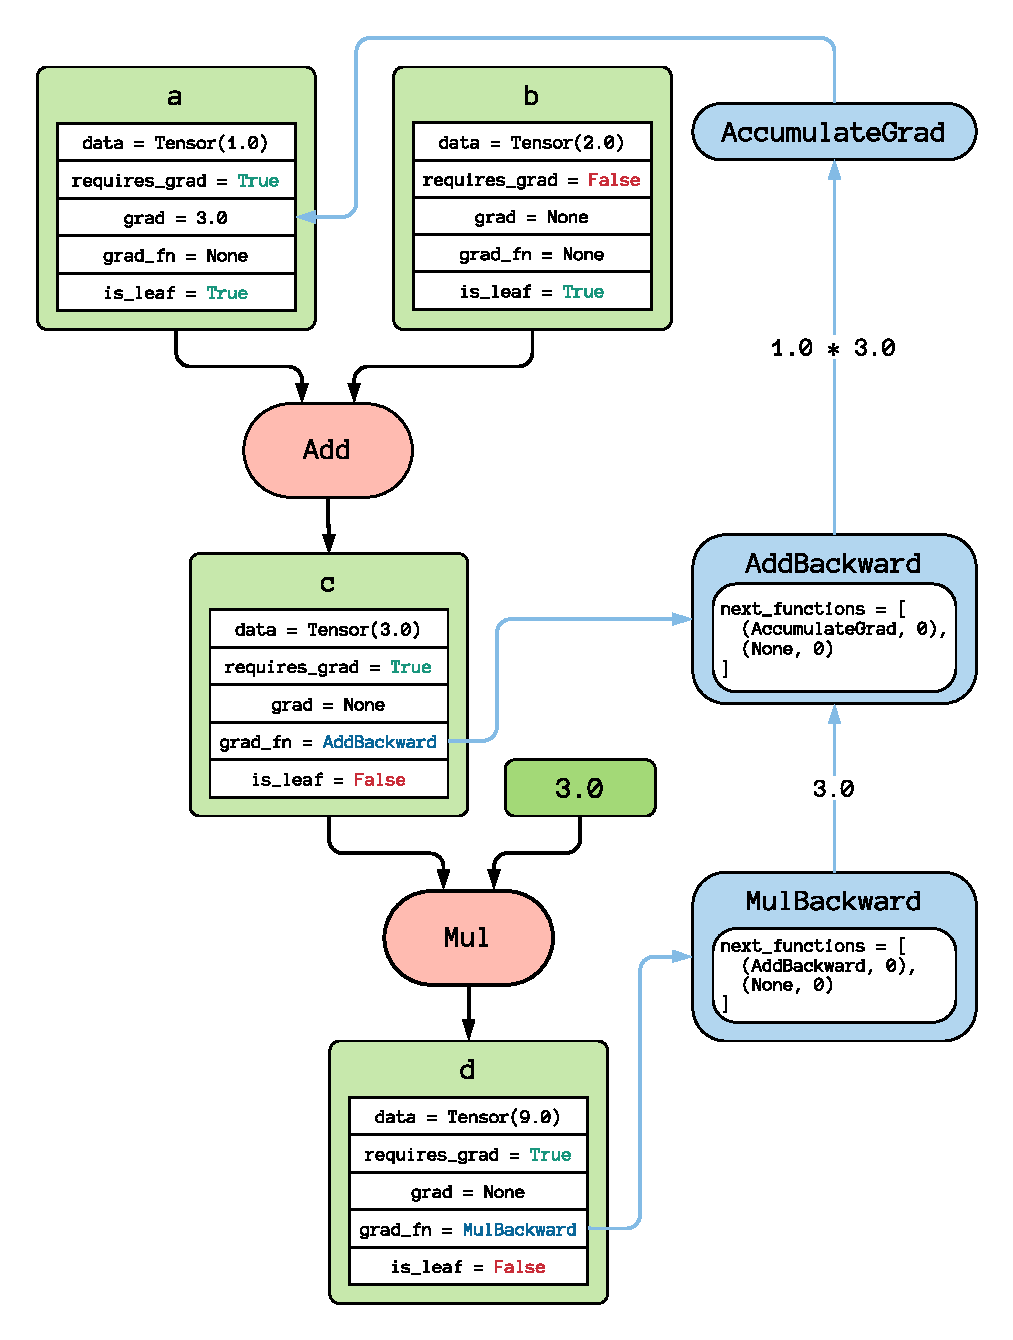
\includegraphics[width=0.9\textwidth]{img/theory/ComputationalGraph.pdf}
    \caption{The computational graph created from the operations in figure \ref{fig:CodeComputationalGraph}. Green nodes represent tensors, red nodes operations and blue nodes the backwards operators that calculate gradients.}
    \label{fig:ComputationalGraph}
\end{figure}

PyTorch operates on its own data structure, called a \codeinline[]{Tensor}, which supports scalars, vectors and matrices of any dimension, much like a Numpy \codeinline[]{ndarray}. Every PyTorch operation performed on a Tensor is registered and added to a directed acyclic graph, usually referred to as a Computational Graph, that tracks the history of computations for that Tensor \cite{autograd}. Each operator in PyTorch extends the \codeinline[python]{Function} class which requires it to implement a \codeinline[python]{forward} and \codeinline[python]{backward} method. The \codeinline[]{forward} performs the operation and the \codeinline[]{backward} method performs the differentiation of the operation. Calling \codeinline[]{backward()} directly on a Tensor will traverse the computational graph in reverse order, using the output of \codeinline[]{backward()} as input to the parent operation, and save the gradient of each participating Tensor in their \codeinline[]{.grad} attribute. An example if shown in figure \ref{fig:ComputationalGraph}, where a few Tensors are created, some operations are performed on them and then the gradient is calculated by calling \codeinline[]{backward()}.

\begin{figure}[h]
    \centering
    \begin{minted}{python}
    a = torch.tensor(1., requires_grad=True)
    b = torch.tensor(2.)
    c = a + b
    d = c * 3.
    d.backward()
    print(d)  # tensor(9.0)
    print(a.grad)  # tensor(3.0)
    \end{minted}
    \caption{}
    \label{fig:CodeComputationalGraph}
\end{figure}

In a way, the backwards traversal of the computational graph is nothing more than a rigorous way of using the standard derivation chain rule, shown in equation \ref{eq:ChainRule}.

\begin{equation}\label{eq:ChainRule}
    \frac{d f(g(x))}{dx} = \frac{d f}{dg} \times \frac{d g}{d x}
\end{equation}

In figure \ref{fig:ComputationalGraph}, we show the computational graph that is created as a result of the operations in \ref{fig:CodeComputationalGraph}. Green color represents Tensor variables, red color represents PyTorch operators while blue color represents everything related to the backward pass that calculates the gradient. Now $\frac{\partial d}{\partial a}$ can automatically be calculated, i.e., the gradient (or more correct the partial derivative) of $d$ with respect to $a$. In the green nodes, the \texttt{requires\_grad} field dictates if a gradient should be computed for this tensor, the \texttt{grad} field contains the calculated gradient value and the \texttt{grad\_fn} contains the backwards version of the last operator used on a tensor. In PyTorch, any tensor explicitly created by the user is called a leaf, denoted by the \texttt{is\_leaf} attribute. Tensors created as a result of operators are not leaves, and PyTorch does not calculate gradients for them. The blue nodes contain a field called \texttt{next\_function} which is a list of tuples that tracks the next backward function to be called. When \texttt{backward()} is called on $d$, the flow backward is started. For Tensors with \codeinline[python]{requires_grad = False} or non-tensors, the next function is None, as we do not need to calculate their gradient. Calculation of the derivative $\frac{d d}{d c} = 3.0$ is already defined in the \texttt{Sum} operator and is passed along to \texttt{AddBackward}. No gradient is passed to tensor $c$ as it is not a leaf. As $b$ has \codeinline[]{requires_grad=False} the next function for $b$ is \texttt{None}. For $a$ however, it is a special function \texttt{AccumulateGrad} that simply accumulates and sets the gradient for $a$. Same as for \texttt{Sum}, \texttt{Add} already contains a definition for its gradient so $\frac{\partial c}{\partial a}$ is easily calculated as $1.0$. Now, according to the chain rule, $\frac{\partial d}{\partial a} = \frac{\partial d}{\partial c} \cdot \frac{\partial c}{\partial a}$, and so we get the product as $1.0 \cdot 3.0$ which is set as the gradient for $a$.

Because PyTorch builds this graph separately for each Tensor, and rebuilds after every call to \texttt{backward()} its possible to use arbitrary Python control flow, like \codeinline[]{for} and \codeinline[]{if} statements, in conjunction with PyTorch operators that can be different for each iteration. This allows us to split our rendering and loss calculations into multiple different processes, as shown in algorithm \ref{alg:GradientDescent}, but still only call \codeinline[]{backward()} on the loss result. Note that this explanation is specific to PyTorch, as not all frameworks implement their computational graph in the exact same way, but most of them follow the same principles.

% \subsection{Vector-Jacobian product}
% The PyTorch operators accept Tensors of arbitrary shape, and so the general case, we want to find the gradient of a \textit{vector valued} function. Given a function $\vec{y} = f(\vec{x})$ where $\vec{x}=(x_0,x_1,...,x_n)$ and $\vec{y} = (y_0,y_1,...,y_m)$ the gradient of $f$ is a so called \textit{Jacobian Matrix}, which is a matrix of all possible partial derivatives of the two vectors $\vec{x}$ and $\vec{y}$, see equation \ref{eq:JacobianMatrix}.

% \begin{equation}\label{eq:JacobianMatrix}
%     \nabla f = J = 
%     \begin{bmatrix} \frac{\partial y_0}{\partial x_0} & \frac{\partial y_0}{\partial x_0} & \dots & \frac{\partial y_0}{\partial x_n} \\ 
%     \frac{\partial y_1}{\partial x_0} & \frac{\partial y_1}{\partial x_1} & \dots & \frac{\partial y_1}{\partial x_n} \\
%     \vdots & \vdots & \ddots & \vdots \\ 
%     \frac{\partial y_m}{\partial x_0} & \frac{\partial y_m}{\partial x_n} & \dots & \frac{\partial y_m}{\partial x_n}
%     \end{bmatrix}
% \end{equation}

% The vector-Jacobian product is the product of a vector $v=(v_0,v_1...v_n)$ and the Jacobian matrix $v^T \cdot J$ and generally, the \texttt{autograd} package of PyTorch is an engine for computing this product.

% Going back to figure \ref{fig:ComputationalGraph}, we call the multiplication operator $mul$ and the addition operator $add$.  We can rewrite rewrite our mathematical notation of $d=(a+b)*3$ in a more programmatical syntax \codeinline[]{d = mul(add(a,b),3)}. To calculate the derivative of $d$, we use the chain rule as shown in equation \ref{}

% \begin{equation}\label{eq:ChainRuleExample}
%     \begin{aligned}
%     \frac{d}{d}mul(add(a,b),3) = \frac{d mul}{d add} \prod \frac{d add}{}
%     \end{aligned}
% \end{equation}

% \textbf{CITE autograd!} \cite{autograd}

\section{Stochastic Gradient Descent}\label{sec:StochasticGradientDescent}

The gradient descent algorithm is one of the cornerstones of this project and is in fact a fairly simple algorithm for iteratively optimizing a, usually, multivariate function. Its most well known use case is in Machine Learning where it is used to minimize the loss of a neural network model. It works by iteratively finding the direction of steepest descent, leading to a minimal value of the loss, defined as the negative of a function's gradient. To find the gradient of a function $f$, it needs to be differentiable which is why our loss function (and each function it depends on) is defined in an auto differentiation framework such as \textit{PyTorch}, see section \ref{sec:AutomaticDifferentiation}.

There are a few major versions of the gradient descent algorithm, the most commonly used in machine learning being mini-batch gradient descent, where the gradient is calculated as an average of multiple samples in order to take a single step. Stochastic gradient descent on the other hand, performs one step for each sample, which is used in our implementation as we only have a single sample (a user's input image). The general algorithm of gradient descent is presented in pseudo-code in algorithm \ref{alg:GradientDescent}. Starting with an arbitrary parameter set $\theta \in \mathbb{R}^n$ which contains all $n$ parameters needed to define an output procedural texture, as well as a loss function $L$ with $\nabla L$ denoting the gradient of $L$ with respect to each parameter in $\theta$, we can update our parameters in each iteration $t$ like shown in equation \ref{eq:GradientDescentUpdate}

\begin{equation}\label{eq:GradientDescentUpdate}
    \begin{aligned}
    v_t = \alpha \cdot \nabla L(\theta_t) \\
    \theta_{t+1} = \theta_t - v_t
    \end{aligned}
\end{equation}

The variable $\alpha \in [0,1]$ is called the learning rate and controls how fast $\theta$ will converge toward the optimal parameter set $\theta^*$ that minimizes our loss function $L$. In general, the gradient descent algorithm solves the optimization problem posed in equation \ref{eq:GradientDescentOptimization}.

\begin{equation}\label{eq:GradientDescentOptimization}
    \argmin_{\theta} L(\theta) = \left\{\theta \mid L(\theta) = \min_{\theta^*} L(\theta^*)\right\}
\end{equation}


The strategy for updating the parameters can be done in much more refined ways using a different \textit{Optimizer}, see section \ref{sec:Optimizer}.  As seen in the algorithm pseudocode and briefly explained in \ref{sec:ComputationalGraph}, we don't actually need the loss to take the set of parameters as input, thanks to the way \textit{PyTorch} registers operations done on any tensor in the set $\theta$ separately for each parameter. 




\begin{algorithm}[H]
\SetKwData{L}{loss}\SetKwData{Iter}{iter}\SetKwData{Truth}{truth}\SetKwData{RenderedImage}{render}
\SetKwFunction{Loss}{Loss}\SetKwFunction{Optimize}{Optimize}\SetKwFunction{Render}{Render}
\SetKwInOut{Input}{Input}\SetKwInOut{Output}{output}

\KwResult{Optimal set of parameters $\mathds{P^*}$ that minimizes loss function \Loss{}}
\Input{The loss goal $l_{goal}$, maximum number of iterations $i_{max}$, and a ground truth image \Truth}

\BlankLine
randomly or strategically initialize $\theta$\;
initialize \Iter $\leftarrow$ $0$\;
\While{\Iter $<$ $i_{max}$}{
    \RenderedImage $\leftarrow$ \Render($\theta$)\;
    \L $\leftarrow$ \Loss{\Truth, \RenderedImage} \;
    \If{\L $\leq$ $l_{goal}$}{
        \Return $\theta$\;
    }
    Backpropagate \L to find the gradient of each parameter in $\theta$\;
    Update $\theta$ according to strategy in optimizer $\theta\leftarrow$\Optimize{$\theta$, $\nabla\theta$}\;
    \Iter $\leftarrow$ \Iter $+1$\;
}
\Return $\theta$\;
\caption{Gradient Descent Algorithm}\label{alg:GradientDescent}
\end{algorithm}


\subsection{Optimizers}\label{sec:Optimizer}

\begin{enumerate}
    \item Insert an image showing SGD oscillating in one direction and the effects momentum has on it, while also explaining why we plot for two variables as a surface plot! \href{https://ruder.io/optimizing-gradient-descent/index.html#gradientdescentoptimizationalgorithms}{LINK}
\end{enumerate}

Optimizers are algorithms describing a strategy for gradient descent to reliably reach the most optimal value of the loss in the fewest amount of steps possible. This is achieved by controlling the updating of the parameters in such a way that we take the largest steps possible towards the optimal value of the loss, without overshooting it or getting stuck in local minima. An analogy of a ball rolling towards the lowest point on a surface (the loss function) in the direction of the downward slope is often used to describe an optimizer's progress. Given a loss function $L$, the most basic optimizer updates each parameter in $\theta$ according to equation \ref{eq:GradientDescentUpdate}. Additionally, for each iteration $t$, the learning rate is usually updated by multiplying it with a decay term $\delta$ so that it diminishes over time. This is to prevent it from overshooting the minimum by forcing it to take smaller steps the closer it gets to the minimum. The drawback of this simple solution, is that it is not very adaptive, and uses the same learning rate for all parameters, thus will give us problems when the derivative differs between parameters. To overcome this, optimizers usually implement something called \textit{momentum}, which adds a fraction $0 \leq \beta \leq 1$ of past update vectors to the current update vector $v_t$. The update steps now become:

\begin{equation}
    \begin{aligned}
    v_t = \beta v_{t-1} + \alpha \cdot \nabla L(\theta) \\
    \theta_{t+1} = \theta_t - v_t
    \end{aligned}
\end{equation}

This is effectively an exponentially weighted moving average, and so for parameters where the gradient is oscillating, this addition will average out those oscillations \textbf{shown in image...}. However, each parameter $\theta_i$ still gets updated using the same learning rate $\alpha$. To battle this, an additional term dubbed \textit{second moment} is calculated, which is a squared weighted average of the past gradients, popularized by \textit{Adagrad} \cite{duchi_2011_adaptive} and refined in \textit{Adadelta} \cite{zeiler_2012_adadelta}. The combination of momentum (first moment) and second moment is used in \textit{Adam} or \textit{Adaptive Moment Estimation}, one of the most popular and successful optimization algorithms used in machine learning \cite{kingma_2014_adam}. The first $m_t$ and second $v_t$ moments for an iteration $t$ are calculated in equation \ref{eq:FirstSecondMoment}.

\begin{equation}\label{eq:FirstSecondMoment}
    \begin{aligned}
    m_t = \beta_1 m_{t-1} + (1-\beta_1) \cdot \nabla L(\theta) \\
    v_t = \beta_2 v_{t-1} + (1 - \beta_2) \cdot \nabla L(\theta)^2
    \end{aligned}
\end{equation}

The two parameters $0 \leq \beta_1, \beta_2 \leq 1$ are used to tune how fast the influence of previous iterations should decay, and is recommended by the authors to be set to $\beta_1 = 0.9$ and $\beta_2 = 0.999$. The second moment, which is a running average of the square of the gradients, controls how much effect the learning rate $\alpha$ has on each parameter $\theta_i$, as shown in equation \ref{eq:Adam}.

\begin{equation}\label{eq:Adam}
    \theta_{t+1} = \theta_t - \frac{\alpha}{\sqrt{v_t} + \epsilon}m_t
\end{equation}

The $\epsilon$ is a small corrective term to prevent division by zero errors. Note that all variables, except $\epsilon$ and $\alpha$ are vectors of size $n$, the number of parameters in $\theta$ and all operations are performed element-wise. Before the first iteration, $m_t$ and $v_t$ are initialized to all zeros, which introduces a bias towards zero for the early iterations. To prevent this, $m_t$ and $v_t$ in equation \ref{eq:Adam} are replaced with their bias corrected versions, $\hat{m}_t$ and $\hat{v}_t$, which are calculated in equation \ref{eq:BiasCorrectedMoments}.

\begin{equation}\label{eq:BiasCorrectedMoments}
    \begin{aligned}
    \hat{m}_t = \frac{m_t}{1- \beta_1^t} \\
    \hat{v}_t = \frac{v_t}{1 - \beta_2^t}
    \end{aligned}
\end{equation}

As the iteration counter $t$ increases, the denominator $1 - \beta^t$ converges towards $1$ and will thus have a negligible effect on the moments in later iterations. Most other optimizers build on these concepts.

\section{Loss functions}

Gradient descent is commonly used to minimize a function that measures the difference between a ground truth $X$, the target, and a generated sample $\hat{X}$, our prediction, as a real number. Such a function is often referred to as a \textit{loss function} or \textit{cost function} as it represents a penalty that we desire to be as small as possible. In our case, we can use it to measure the difference between a user input texture image, our target, and an image that our system has generated. A loss function should output a single scalar value, where larger values represent a bigger difference and a value of zero represent two identical images, at least as measured by the loss function. In general, a loss function could have any input, but our implementations follow what is shown in equation \ref{eq:LossFunctionMapping}, where $L$ denotes a loss function that maps an input of two images matrices $\hat{X}$ and $X$ to a real scalar value. The matrices are real valued and in \textit{column-first} order which is why the width is specified first in $\mathbb{R}^{w \times h \times 3}$, where $w$ and $h$ is the width and height of a rendered image with three color channels.

\begin{equation}
    \begin{aligned}
    L: \hat{X},X \mapsto \mathbb{R} \\
    \text{where } \hat{X}, X \in \mathbb{R}^{w\times h \times 3} \text{ and } w, h \in \mathbb{N}
    \end{aligned}
    \label{eq:LossFunctionMapping}
\end{equation}

The choice of loss function wholly depends on what is being measured. Loss functions for images are a special case, and an entire field of research on its own. Often, it is desired to design a loss function in a way that coincides with a human's perceived difference of two images which can be difficult as the human visual system is very complex. Often simple losses, like MSE explained in section \ref{sec:MeanSquaredError}, are very sensitive to spatial changes in data, which is why more advanced losses are often required.

\subsection{Mean Squared Error}\label{sec:MeanSquaredError}

Mean Squared Error is a popular and simple loss function that measures the squared difference of each pixel, sums them and returns the mean of the sum as shown in equation \ref{eq:MSE}. This kind of loss function is useful if the goal is to reproduce the target image down to the pixel. This is however, not a good representation of how a human would judge the similarity of two images. If target image $X$ and predicted image $\hat{X}$ are identical, except each pixel in $\hat{X}$ is shifted one column to the right, it would still be very hard to distinguish any difference between the two for a human (given a reasonable resolution). Depending on the amount of noise in the image, almost no pixels are identical anymore and we get a large measured difference. This also applies to any scaling, rotation or sheering of images. Thus, MSE has a strong spatial dependency on the compared images. Especially in this project, where procedural textures with high frequency features and patterns is common, we need to look for more sophisticated means of measuring differences between images.

\begin{equation}\label{eq:MSE}
    L_{mse}(\hat{X}, X) = \frac{1}{w\cdot h\cdot 3}\sum_{i,j,c} (\hat{X}_{i,j,c} - X_{i,j,c})^2
\end{equation}

\subsection{Neural Feature Loss}

\begin{enumerate}
    \item Describe how features are extracted and what a gram matrix is...
    \item \textbf{Insert image from lucidchart showing features being extracted...}
    \item Mention that these neural losses are input to MSE.
\end{enumerate}

Developing a reliable method of measuring differences in images is important in inverse graphics as well as machine learning and directly influences its performance. In a way, our algorithm is only as good as our loss function, defining an upper bound on accuracy. In the paper by Guo et. al \cite{guo_2019_a}, several different loss functions are discussed, reaching the conclusion that a loss utilizing features extracted by a neural network such as VGG19 \cite{simonyan_2015_very} performed best. This method is directly adapted from a paper by Gatys et. al. \cite{gatys_2015_texture}, where feature maps $F_i$ are extracted from a few layers of VGG19, and then multiplied together to obtain a \textit{Gram Matrix}. Hu et. al. also used a verion of this as the loss for their neural network model, but calculated histograms on the features instead \cite{hu_2019_a}. Some of these methods are implemented and tested in our project.

\section{Related work}

This thesis primarily cover two topics; Inverse Rendering and Procedural Textures. Neither subjects are new and are both well researched but few papers attempt to combine the two topics. Many approaches at inverse rendering use neural networks, with good results for their somewhat narrow use cases. This thesis was born from inspiration of this method, but it was soon discovered that it is not a viable solution for our use case, where we allow users to freely modify and compose procedural textures, resulting in near endless pattern combinations. Training a neural network to perform well on such data would require an immense dataset to train on, as well as an extremely complex model.

\subsection{Inverse Graphics using Neural Networks}

A popular approach to the inverse graphics problem is using neural networks. Kulkarni et. al propose using a modified Variational Auto Encoder to learn disentangled 3D transformation properties (such as rotation about an axis, or the azimuth of the light source) of a 3D scene \cite{kulkarni_2015_deep}. A \textit{disentangled} representation means that each latent variable $z_i$ in the VAE represents a distinct transformation of the 3D scene. This is achieved, in part, by traning on batches of images where all but one parameter are kept constant. A similar approach is used in a paper by Mahendran et. al, although using a convolutional neural network \cite{mahendran_2017_3d} while a third solution is to use a Generative Adversarial Network that imitates a graphics renderer, which Shi et. al recently did to retrieve parameters for 3D faces from 2D images \cite{shi_2019_facetoparameter}. Neither of these solutions specialize in inverse rendering of textures, but instead a small subset of possible 3D scene parameters or in the case of Shi et. al. a pre-defined set of 3D face parameters. This approach can be adapted for simple pre-defined procedural textures, but is difficult to train on more complex examples. Neural networks also requires a lot of preparation, such as generating training data and requires pre-designed textures and are therefore not a flexible solution.

\subsection{SVBRDF Aquisition}

SVBRDF aquisiton is a popular subsection of inverse graphics for textures that focus on decomposing 2D image textures into spatially-varying bi-directional reflectance distribution functions (SVBRDF for short) maps that describe a texture's roughness, specularity or 3D displacement (normal map) etc. Many papers have in recent years used different neural networks models or image analysis to achieve this \cite{deschaintre_2018_singleimage, kang_2018_efficient, nalbach_2017_deep, aittala_2016_reflectance}. However, instead of finding these maps directly, our thesis focuses on finding the parameters to a procedural texture that allows us to modify it and generate it, albeit only a limited subset of these maps, as we do not consider any 3D displacement or light interaction in this thesis.

\subsection{Texture Synthesis}

Texture synthesis is a very active research area where a sample image is used to create a larger texture with the same pattern and style. Virtually all texture synthesis solutions work with bitmap textures, and thus act as an alternative solution to procedural textures when the goal is to generate varied larger textures from a sample. Solving the inverse problem is not very common, nor is it often needed as it is usually easier to acquire a small texture example of a desired larger version. None the less, Wei et. al. managed to create a framework for inverse texture synthesis, and argued that that it is useful for acquiring a sample from inhomogenous textures \cite{wei_2008_inverse}. Some early solutions to texture synthesis relied on feature extraction and optimization between input and output texture \cite{kwatra_2005_texture}, while others utilized a patch based method where a new image is created by stitching together patches of the original sample \cite{efrosalexeia_2001_image}. As the popularity of neural networks grew, the field of texture synthesis found itself moving away from more manual image analysis solutions and started utilizing CNNs and later GANs. Early on, Gatys et. al. proposed a method for texture synthesis based on extracting features from different levels of a neural network \cite{gatys_2015_texture}. However, recent papers have found that GANs can be used to create high quality results of impressive resolutions. Notably, Früstück et. al. created a framework that supports multiple example images as input to produce a large-scale texture with very little boundary artefacts \cite{frhstck_2019_tilegan}. While texture synthesis can be used to quickly generate high quality output, they are still bound to the pixel space and will thus consume large amounts of storage space and lack the flexibility of being easily modifyable, much like SVBRDF maps.


\subsection{Inverse Procedural Texture Modeling}

This field of computer science is rather specific and a relatively low amount of research has been done on it. Two very recent papers stand out as perhaps the most related work of all, and have been the foundation of this thesis. In 2019, Hu et. al. published \textit{A Novel Framework For Inverse Procedural Texture Modeling} in which they describe a framework for procedural texture model acquisition as well as parameter estimation for said model \cite{hu_2019_a}. A K-means algorithm is used to find the most suitable procedural texture model, among a library of pre-defined models, for a user's input texture. Each procedural texture model has an associated CNN model which is used to solve the regression problem of finding an optimal parameter set to the procedural texture that renders an image close to the users input image. This approach is unfortunately not very flexible, as the procedural textures have to be pre-defined and training a neural network on each texture requires a considerable amount of effort and time. Using CNNs for regression also proved difficult for complex procedural texture models, and so neural networks were abandoned for this thesis altogether. 

A much different approach was formulated in the work by Guo et. al. in 2019, where their solution involves Bayesian inference and sampling of the space of plausible parameters to find an optimal parameter set for a chosen procedural texture \cite{guo_2019_a}. Their solution of an approach implemented in a differentiable framework like \textit{PyTorch} is a direct inspiration, however, in our approach no sampling is needed. Furthermore, they contribute by developing smart loss functions that do not depend on textures being pixelwise aligned which have been implemented in this thesis. One defining differece between their work and ours, is that they do not provide an interface to create procedural textures, and only offers hard-coded procedural textures.

\subsection{Differentiable Rendering}

An important foundation that allows our approach to work is the concept of differentiable rendering, that is, the ability to differentiate the entire rendering process, and thus obtain gradients for it. A few notable examples of this have been an inspiration when we write our own differentiable renderer. Perhaps most notable is the very recently released PyTorch3D, a rendering framework developed by the team behind \textit{PyTorch} \cite{facebookresearch_2020_facebookresearchpytorch3d, paszke_2019_pytorch}. This renderer is in fact implemented in \textit{PyTorch}, making it fully differentiable. This tool was unfortunately released without our knowledge at the same time as this thesis was started, but share many concepts, although their approach is much more general. If time allows, it would be worthwile implementing the rendering of this project in their framework. Earlier approaches like the OpenDR framework is closely related to our project, but with a different focus \cite{loper_2014_opendr}. Similar to our project they create a framework where the entire forward rendering process is differentiable, enabling it to automatically compute scene parameters such as vertex positions, camera parameters and vertex colors. Our solution does not focus on the 3D model or camera parameters, but on per-pixel procedural colors and not only static vertex colors. As much of our algorithm relies on writing differentiable shaders, we must not fail to mention an attempt to do just that, directly implemented in the HLSL shader language \cite{guenter_2011_symbolic}. This project was led by Microsoft Research and although their use case was more aimed towards calculating efficient normals, tangents and derivatives of sub-routines, it remains an interesting idea that sadly would have been too complex to implement in this thesis.